% Chapter Title Page
\clearpage
\thispagestyle{empty} 
\begin{center}
    \vspace*{\fill} 
    \Huge \textbf{Chapter 9} \\
    \Huge \textbf{Public-Key Infrastructure (PKI)}
    \vspace*{\fill}
\end{center}
\clearpage
\fancyfoot[]{}
\chapter{Public-Key Infrastructure (PKI)}

\section{Definition:}
\begin{itemize}
    \item PKI supports the distribution and identification of public encryption keys.
    \item It enables secure data exchange over networks and verifies the identity of the other party.
    \item PKI binds public keys to entities and manages public key bindings.
\end{itemize}

\section{Public-Key Certificates:}
\begin{itemize}
    \item A public-key certificate is a set of data that uniquely identifies an entity, containing the entity’s public key and other data.
    \item It is digitally signed by a trusted party, known as the Certification Authority (CA), binding the public key to the entity.
    \item The certificate solves the problem of public-key distribution by ensuring authenticity.
\end{itemize}

\section{Certificate Generation and Use:}
\begin{itemize}
    \item \textbf{Certificate Components:}
    \begin{itemize}
        \item Contains unique identifying information for the entity.
        \item Public key of the entity.
        \item Information about the CA.
        \item Certificate details (e.g., expiration date).
    \end{itemize}
    \item \textbf{Signing:}
    \begin{itemize}
        \item Information is hashed, and a digital signature is generated using the CA’s private key.
        \item The certificate is signed and can be broadcast or attached to documents.
    \end{itemize}
    \item \textbf{Verification:}
    \begin{itemize}
        \item Users verify the certificate's validity using the CA’s public key.
        \item Ensures the public key in the certificate is authentic.
    \end{itemize}
\end{itemize}
\begin{figure}
    \centering
    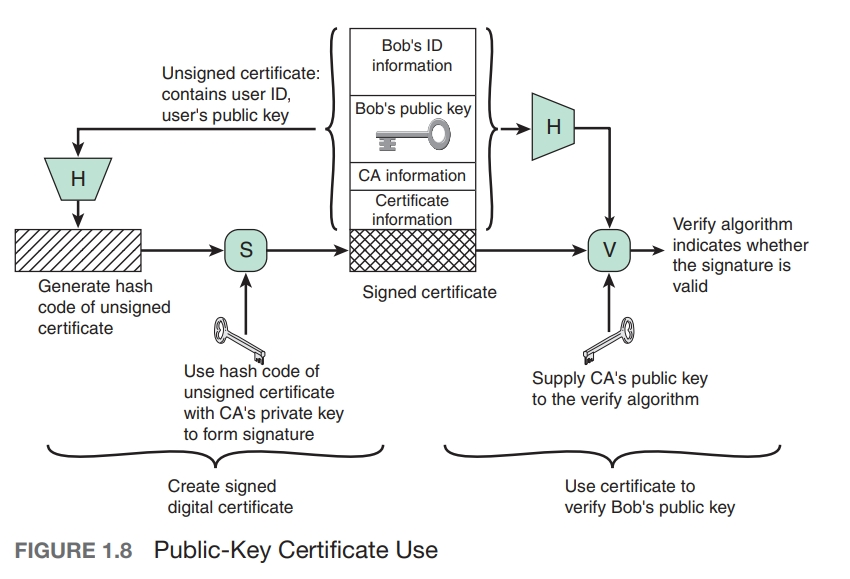
\includegraphics[width=1\linewidth]{Data_Privacy_and_Cryptography/Figures/public key certificate use.jpeg}
    \caption{Public-Key Certificate Use}
    \label{fig:enter-label}
\end{figure}
\section{PKI Architecture:}

\subsection{Requirements:}
\begin{itemize}
    \item Any participant can read and verify a certificate’s owner and authenticity.
    \item Only the CA can create and update certificates.
    \item Participants can verify the current validity of certificates.
\end{itemize}
\begin{figure}
    \centering
    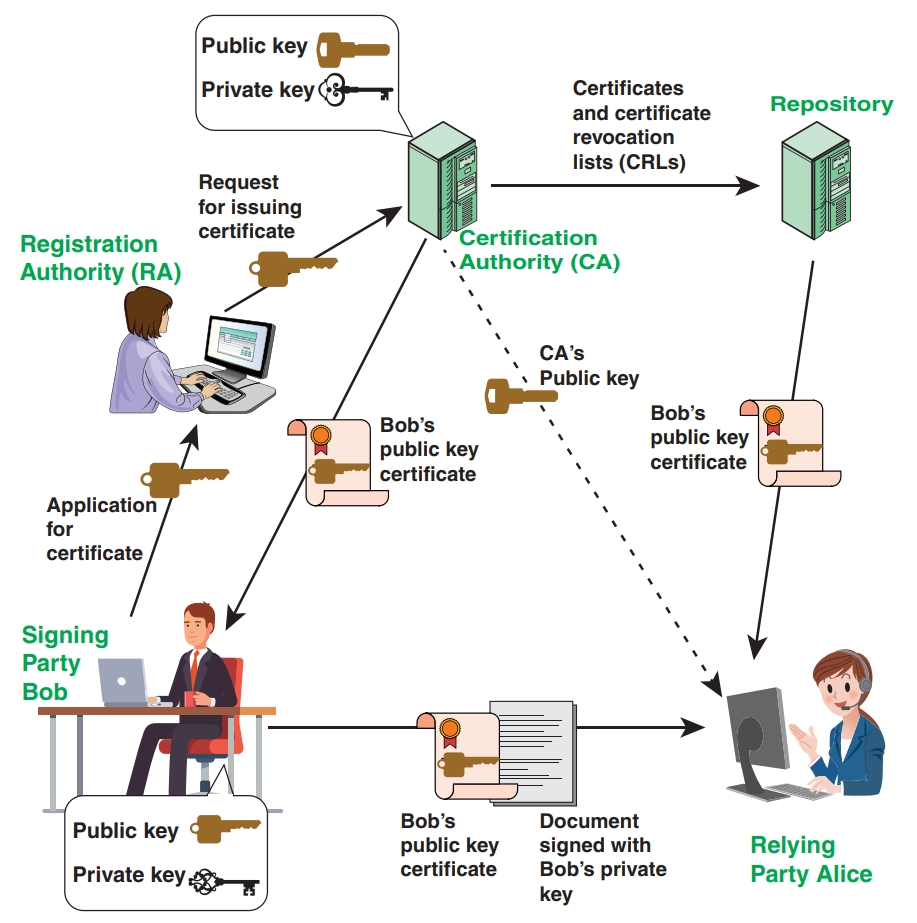
\includegraphics[width=1\linewidth]{Data_Privacy_and_Cryptography/Figures/PKI Scenario.jpeg}
    \caption{PKI Scenario}
    \label{fig:enter-label}
\end{figure}
\subsection{Components:}
\begin{itemize}
    \item \textbf{End Entity:} Users, devices, or processes identified in certificates.
    \item \textbf{Certification Authority (CA):} Creates and assigns certificates, issues certificate revocation lists (CRLs).
    \item \textbf{Registration Authority (RA):} Optional, offloads administrative functions from the CA, verifies end entity identity.
    \item \textbf{Repository:} Stores and retrieves PKI-related information (certificates and CRLs).
    \item \textbf{Relying Party:} Users or agents relying on certificate data for decision-making.
\end{itemize}

\section{Certificate Use Example:}
\begin{itemize}
    \item Alice needs Bob’s public key.
    \item Alice obtains the CA’s public key securely.
    \item Alice checks the repository for Bob’s certificate and verifies its validity.
    \item Alice encrypts data to Bob using Bob’s public key.
    \item Bob can send a signed document to Alice, who verifies the signature with Bob’s public key.
\end{itemize}

\section{Hierarchical CA Organization:}
\begin{itemize}
    \item Multiple CAs can be organized hierarchically, with a root CA signing subordinate CAs.
    \item Root certificates are embedded in browsers and other software for built-in trust.
\end{itemize}
